\documentclass[11pt, ngerman]{scrartcl}

% standard packages
\usepackage[utf8]{inputenc}  % input in UTF-8
\usepackage[T1]{fontenc}  % output in T1 fonts (westeuropäische Codierung)
\usepackage{lmodern}  % latin modern fonts
\usepackage[ngerman]{babel}  % deutsches Sprachpaket, neue Rechtschreibung

% Seitensetup
\usepackage{scrlayer-scrpage}  % Seitenformatierung durch KOMA-interne Optionen
\usepackage[top=4cm, bottom=4cm]{geometry}  % Seitengeometrie (kann durch KOMA ersetzt werden, hab ich aber nicht geschafft)
\usepackage[hypcap=false]{caption, subcaption}  % caption editing - hypcap warning with hyperref
\usepackage{array}  % table editing

% additional packages
\usepackage{amsmath, amssymb, amstext}  % math packages (American Math Society)
\usepackage{bm}
\usepackage{icomma}  % Kommata in Dezimalzahlen verursachen keinen Abstand mehr
\usepackage{graphicx}  % Bilder einfügen
\usepackage{float} %Bilder placement
\usepackage{pdfpages}  % PDF als vollständige Seiten einfügen
\usepackage{lastpage}  % referenziert die letzte Seite
\usepackage[separate-uncertainty=true]{siunitx}  % bessere Darstellung von Einheiten
\usepackage{makecell} %Dicke Tabellenstriche
\usepackage{longtable}
\usepackage{booktabs}
%\usepackage{datatool}
\usepackage[hidelinks]{hyperref}  % hyperref verlinkt Referenzen - hidelinks entfernt borders um links

% package setups
% Kopf- und Fußzeile durch KOMA
\pagestyle{scrheadings}  % KOMA darf entscheiden
\clearpairofpagestyles  % reset
\setkomafont{pageheadfoot}{\normalfont}  % Standardschrift in Kopf- und Fußzeile
\captionsetup{format=plain, font=small, labelfont=bf} %Better caption, Abbildung ist FETT
%\setlength{\headheight}{27.2pt}  % benötigte Höhe Kopfzeile (warning von scrlayer-scrpage, wird aber automatisch so gerendert, falls diese Option weggelassen wird)
\ihead{Kalorimetrie}  % Kopf links %Todo Titel ändern
\chead{\textsc{Philipp} Maximilian}  % Kopf Mitte %Todo Name ändern
\ohead{5 Juni 2021}  % Kopf rechts %Todo Datum ändern
\cfoot{\pagemark \, / \pageref{LastPage}}  % Fuß Mitte

% Table of Contents
\DeclareTOCStyleEntry{dottedtocline}{section}  % KOMA intern - Inhaltsverzeichnis mit Punkten (nur sections)

%Overbar setup
\newcommand{\overbar}[1]{\mkern 1.5mu\overline{\mkern-1.5mu#1\mkern-1.5mu}\mkern 1.5mu}
% SI
\sisetup{locale = DE}  % deutschsprachige SI-Konvention
\sisetup{quotient-mode = fraction}
\sisetup{per-mode = fraction}
\DeclareSIUnit\px{px}
\DeclareSIUnit\permille{\text{\textperthousand}}

% citation
\usepackage{csquotes}
\usepackage[backend=biber]{biblatex}
\addbibresource{kalorimetrie.bib} %Todo .bib befüllen zb.: mit JabRef (Empfehlung der Redaktion)

% array
\renewcommand{\arraystretch}{1.2}

\begin{document}

\title{Kalorimetrie}
\author{\textsc{Philipp} Maximilian\\11839611}
\date{05.06.2021}
\maketitle
%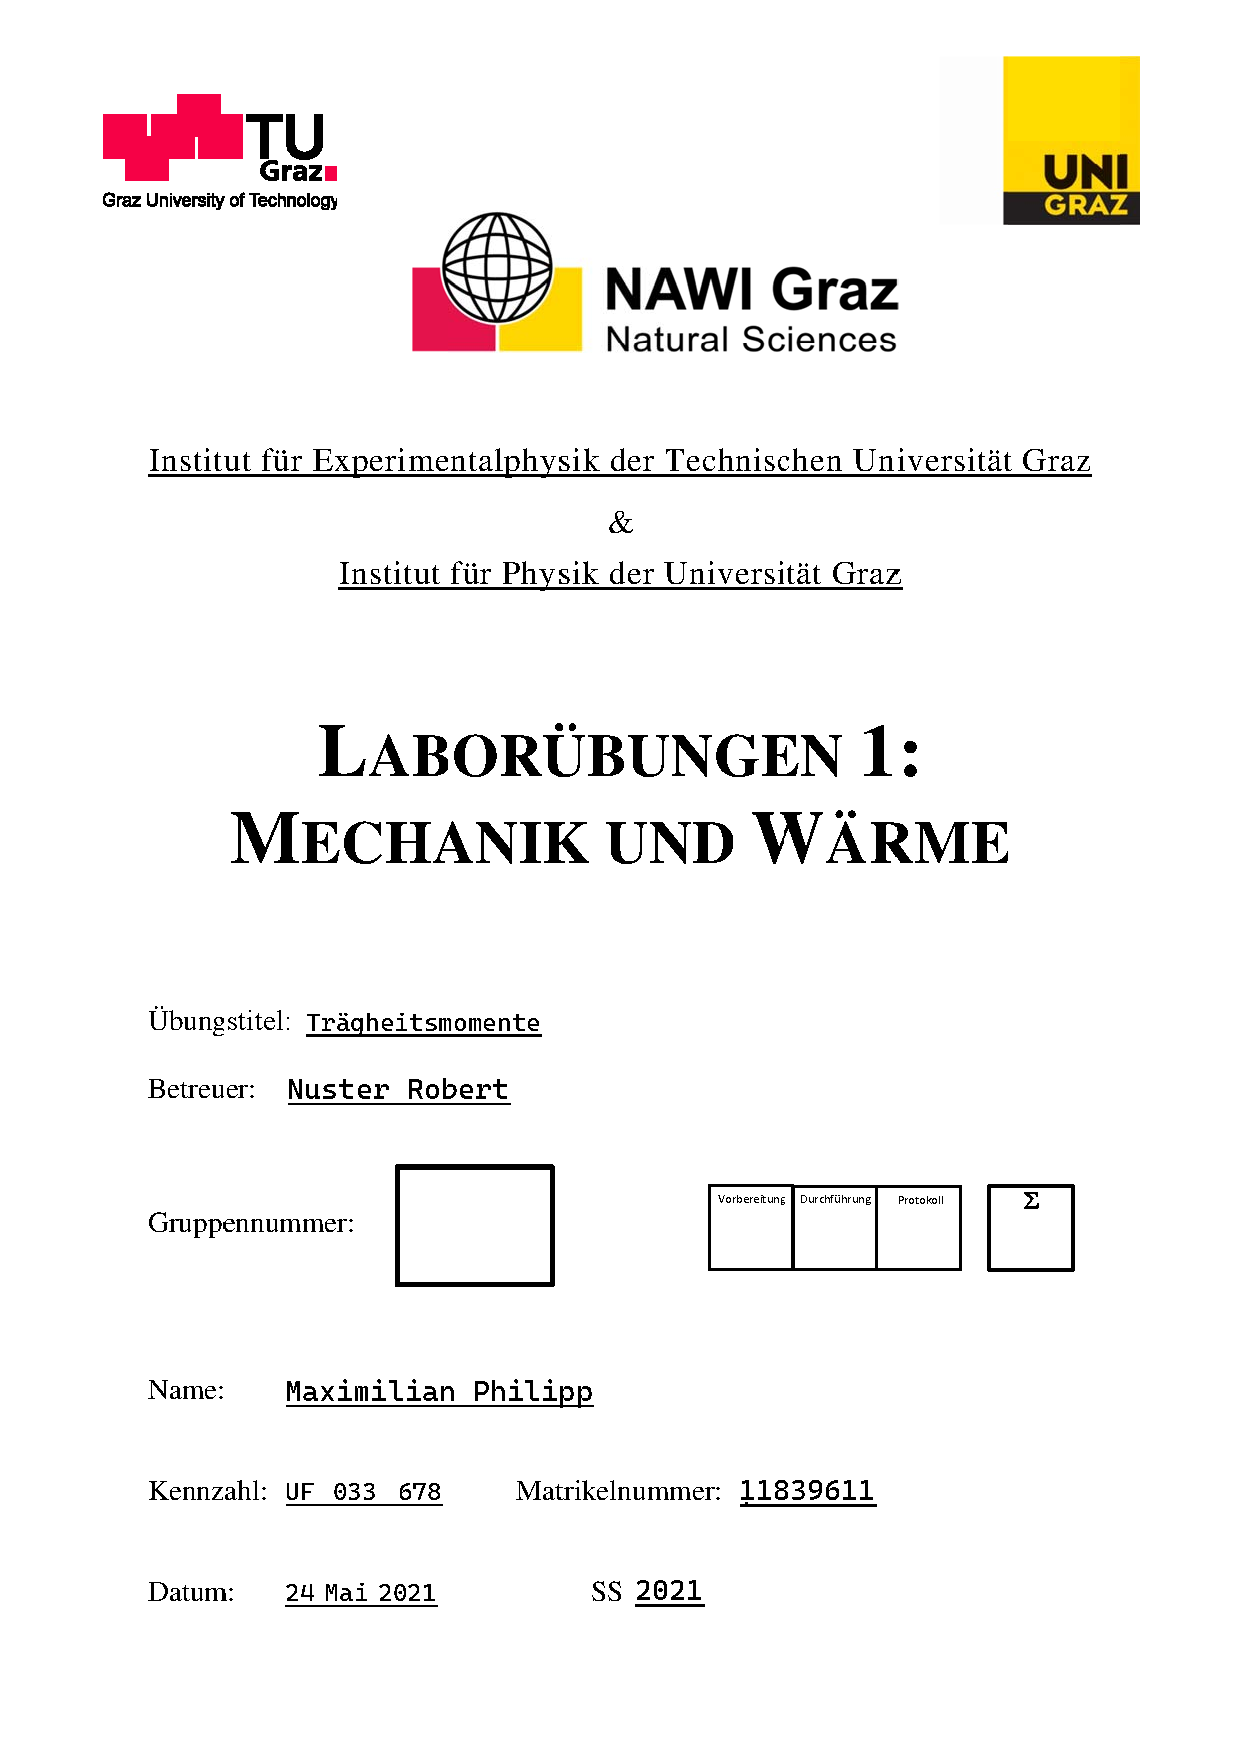
\includepdf{pdfs/Deckblatt.pdf} % Todo Deckblatt ausfüllen

\tableofcontents
\newpage
\section{Aufgabenstellung}
\label{sec:aufgabenstellung}

Die folgenden Punkte sind zu erfüllen:

\begin{enumerate}
	\item Bestimmung der Wärmekapazität $C_K$ des Kalorimeters (eines selbst gebauten Gefäßes)
	\item Für einige ausgewählte Feststoffe (Kartoffeln $c_{Kartoffeln}$, Ethanol $c_{E}$)
	      ist die spezifische Wärmekapazität nach der Mischungsmethode zu ermitteln.
\end{enumerate}

\section{Voraussetzungen und Grundlagen}
\label{sec:voraussetzungen_grundlagen}

Wird die Temperatur $T$ eines Stoffes erhöht, so muss ihm Wärmemenge (Energie) $\Delta Q$
zugeführt werden. Die gesamte, durch die Temperatur geänderte, Energie lässt sich mit der
spezifischen Wärmekapazität $c$ und der Masse $m$ schreiben zu:

\begin{equation}
	\Delta Q = cm \Delta T
\end{equation}

Da im Experiment die Änderung der Temperatur meist bei konstantem Druck erfolgt, soll hier auch die spezifische Wärmekapazität bei konstantem Druck verstanden werden. Werden nun
zwei Stoffe $A$ und $B$ miteinander gemischt, so gilt für die gesamte Wärmemenge:

\begin{equation}
	Q_{A+B} = Q_A + Q_{B}
\end{equation}

Dabei ist eine mögliche Wechselwirkung $Q_{AB}$ vernachlässigt worden. In diesem Fall kann für
die Temperaturänderung der gesamten Wärmemenge

\begin{equation}
	\Delta Q_{A+B} \cong (c_A m_A + c_B m_B) \Delta T
\end{equation}

geschrieben werden. Dieses einfache Ergebnis kann dazu verwendet werden, die
spezifische Wärmekapazität zu bestimmen, wenn mit einem anderen Stoff mit
bekannter Wärmekapazität gemischt wird. Zunächst sollen sich die beiden Stoffe
auf unterschiedlicher Temperatur $T_A$ und $T_B$ befinden. Werden nun beide Stoffe
miteinander gemischt, so stellt sich eine Mischtemperatur $T_m$ ein. Wird dabei
die Mischung in einem abgeschlossenen System durchgeführt, wo die Gesamtenergie
erhalten bleiben muss (Kalorimetergefäß), so kann aus der Gleichsetzung der
Wärmeenergien vor und nach der Mischung die unbekannte spezifische
Wärmekapazität (z.B. $c_A$) berechnet werden. Wird dabei noch berücksichtigt, dass
auch das Kalorimetergefäß eine Wärmekapazität $C_K$ besitzt und vor der Mischung
auf Temperatur $T_B$ ist, so erhält man:

Vor der Mischung: $Q_{A+B} = Q_A + Q_B =  c_A m_A T_A + c_B m_B T_B + C_K T_B$

Nach der Mischung: $Q_{A+B} = Q_A + Q_B = c_A m_A T_m + c_B m_B T_m + C_K T_m$

Da, vor und nach der Mischung, noch die gleiche Wärmemenge vorhanden ist, sind
diese zwei Gleichungen gleich.  Wenn $c_A$ und $c_B$ bekannt oder gleich ($c_W$)
sind, wenn zB. das gleiche Material verwendet wird erhält man folgende Gleichung:

\begin{equation}
	C_K = \frac{c_W m_A (T_A-T_m) + c_W m_B (T_B-T_m)}{T_m-T_B} \label{eq:warmegefaes}
\end{equation}

Somit lässt $C_K$ mit einer bekannten spezifischen Wärmekapazität $c_W$ (zB.
Wasser) und dem Wissen der verschiedenen Temperaturen bestimmen.

Aus $c_A m_A T_A + c_B m_B T_B + C_K T_B = c_A m_A T_m + c_B m_B T_m + C_K T_m$
folgt:

\begin{equation}
	c_A = \frac{(c_B m_B + C_K) (T_B - T_m)}{m_A (T_m - T_A)} \label{eq:warmestoff}
\end{equation}

Wenn $c_B$, $C_K$ und die verschiedenen Temperaturen bekannt sind,
ist es möglich die $c_A$ zu bestimmen.

Um zu sehen wie sich die Unsicherheit der Messungen bis in die Ergebnisse
fortplanzt, ist \autoref{eq:Unsicherheitsfortpflanzung} verwendet worden.
Die Grundlagen dieser Gleichung sind von den Powerpointfolien von
GUM entnommen worden.\cite{WolfgangKessel2004} Die Verallgemeinerung stammt von Wikipedia \cite{2020Fehler}.
Für die Auswertung ist die Progammiersprache Python im speziellen das
Packet \verb#scipy#, zur Hilfe genommen worden.

\begin{equation}
	\label{eq:Unsicherheitsfortpflanzung}
	V_y = J(x) \cdot V_x \cdot J^{T}(x)
\end{equation}

Wobei $V_y$ und $V_x$ die Kovarianzmatrizen von den Vektoren $\bm{y}$ und $\bm{x}$.
$\bm{x}$ ist der Vektor der Eingangsvariablen und $\bm{y}$ ist der Vektor der Ausgangsvariablen.
$J$ ist die Jakobimatrix der vektorwertigen Funktion $\bm{y} = \vec{F}(\bm{x})$.
So lassen sich die Komponenten der Matrix relativ einfach anschreiben $J_{ij}(x) = \frac{\partial{y_i}}{\partial{x_j}}(x)$.
Damit man die Unsicherheit der einzelnen Variablen $y_i$ bekommt, muss nur die Quadratwurzel des i-ten Diagonalelementes der
$\bm{y}$-Kovarianzmatrix genommen werden $u_i= \sqrt{\mathrm{diag}(V_y)_i}$.
Da in diesem Experiment meistens nur skalare Funktionen untersucht werden, vereinfacht
sich die \autoref{eq:Unsicherheitsfortpflanzung} dramatisch und die Unsicherheit
der Variable $y$ lässt sich einfach so berechnen:

\begin{equation}
	\label{eq:graduncentainty}
	u_y = \sqrt{\mathrm{grad} y^T \cdot V_x \cdot \mathrm{grad} y}
\end{equation}

\section{Versuchsanordnung}
\label{sec:versuchsanordnung}

Als Vorbereitung für den Versuch, wurde ein isoliertes Gefäß gebaut, welches
aus einer Plastikflasche besteht, die mittels Bauschaum zu allen Seiten hin
isoliert ist. Diese wurde auf die Waage gestellt, um die Massen
zu messen die dem Gefäß hinzugefügt werden, siehe \autoref{fig:waageaufbau1} oder \autoref{fig:waageaufbau2}. Ein Thermometer ist in
der Nähe zu behalten um die Temperaturen messen zu können.
Damit die Temperatur auch gemessen werden kann, wenn das Gefäß geschlossen
ist, ist die Probe des Thermometers durch den PU-Schaum gestochen worden, siehe
\autoref{fig:aufbauthermo}.


Da es Probleme bei dem Probeversuch beim Messen der spezifischen Wärmekapazität
von Eisen gab, wie es bei den Hinweisen \cite{wärmehinweise} bereits gesagt wurde, wurde entschieden statt Eisen
Kartoffeln als Objekt und Ethanol, wie im Experimentiervorschlag vorgeschlagen,
zu verwenden.


\begin{figure}[H]
	\centering
	\begin{minipage}[t]{.33\linewidth} % [b] => Ausrichtung an \caption
		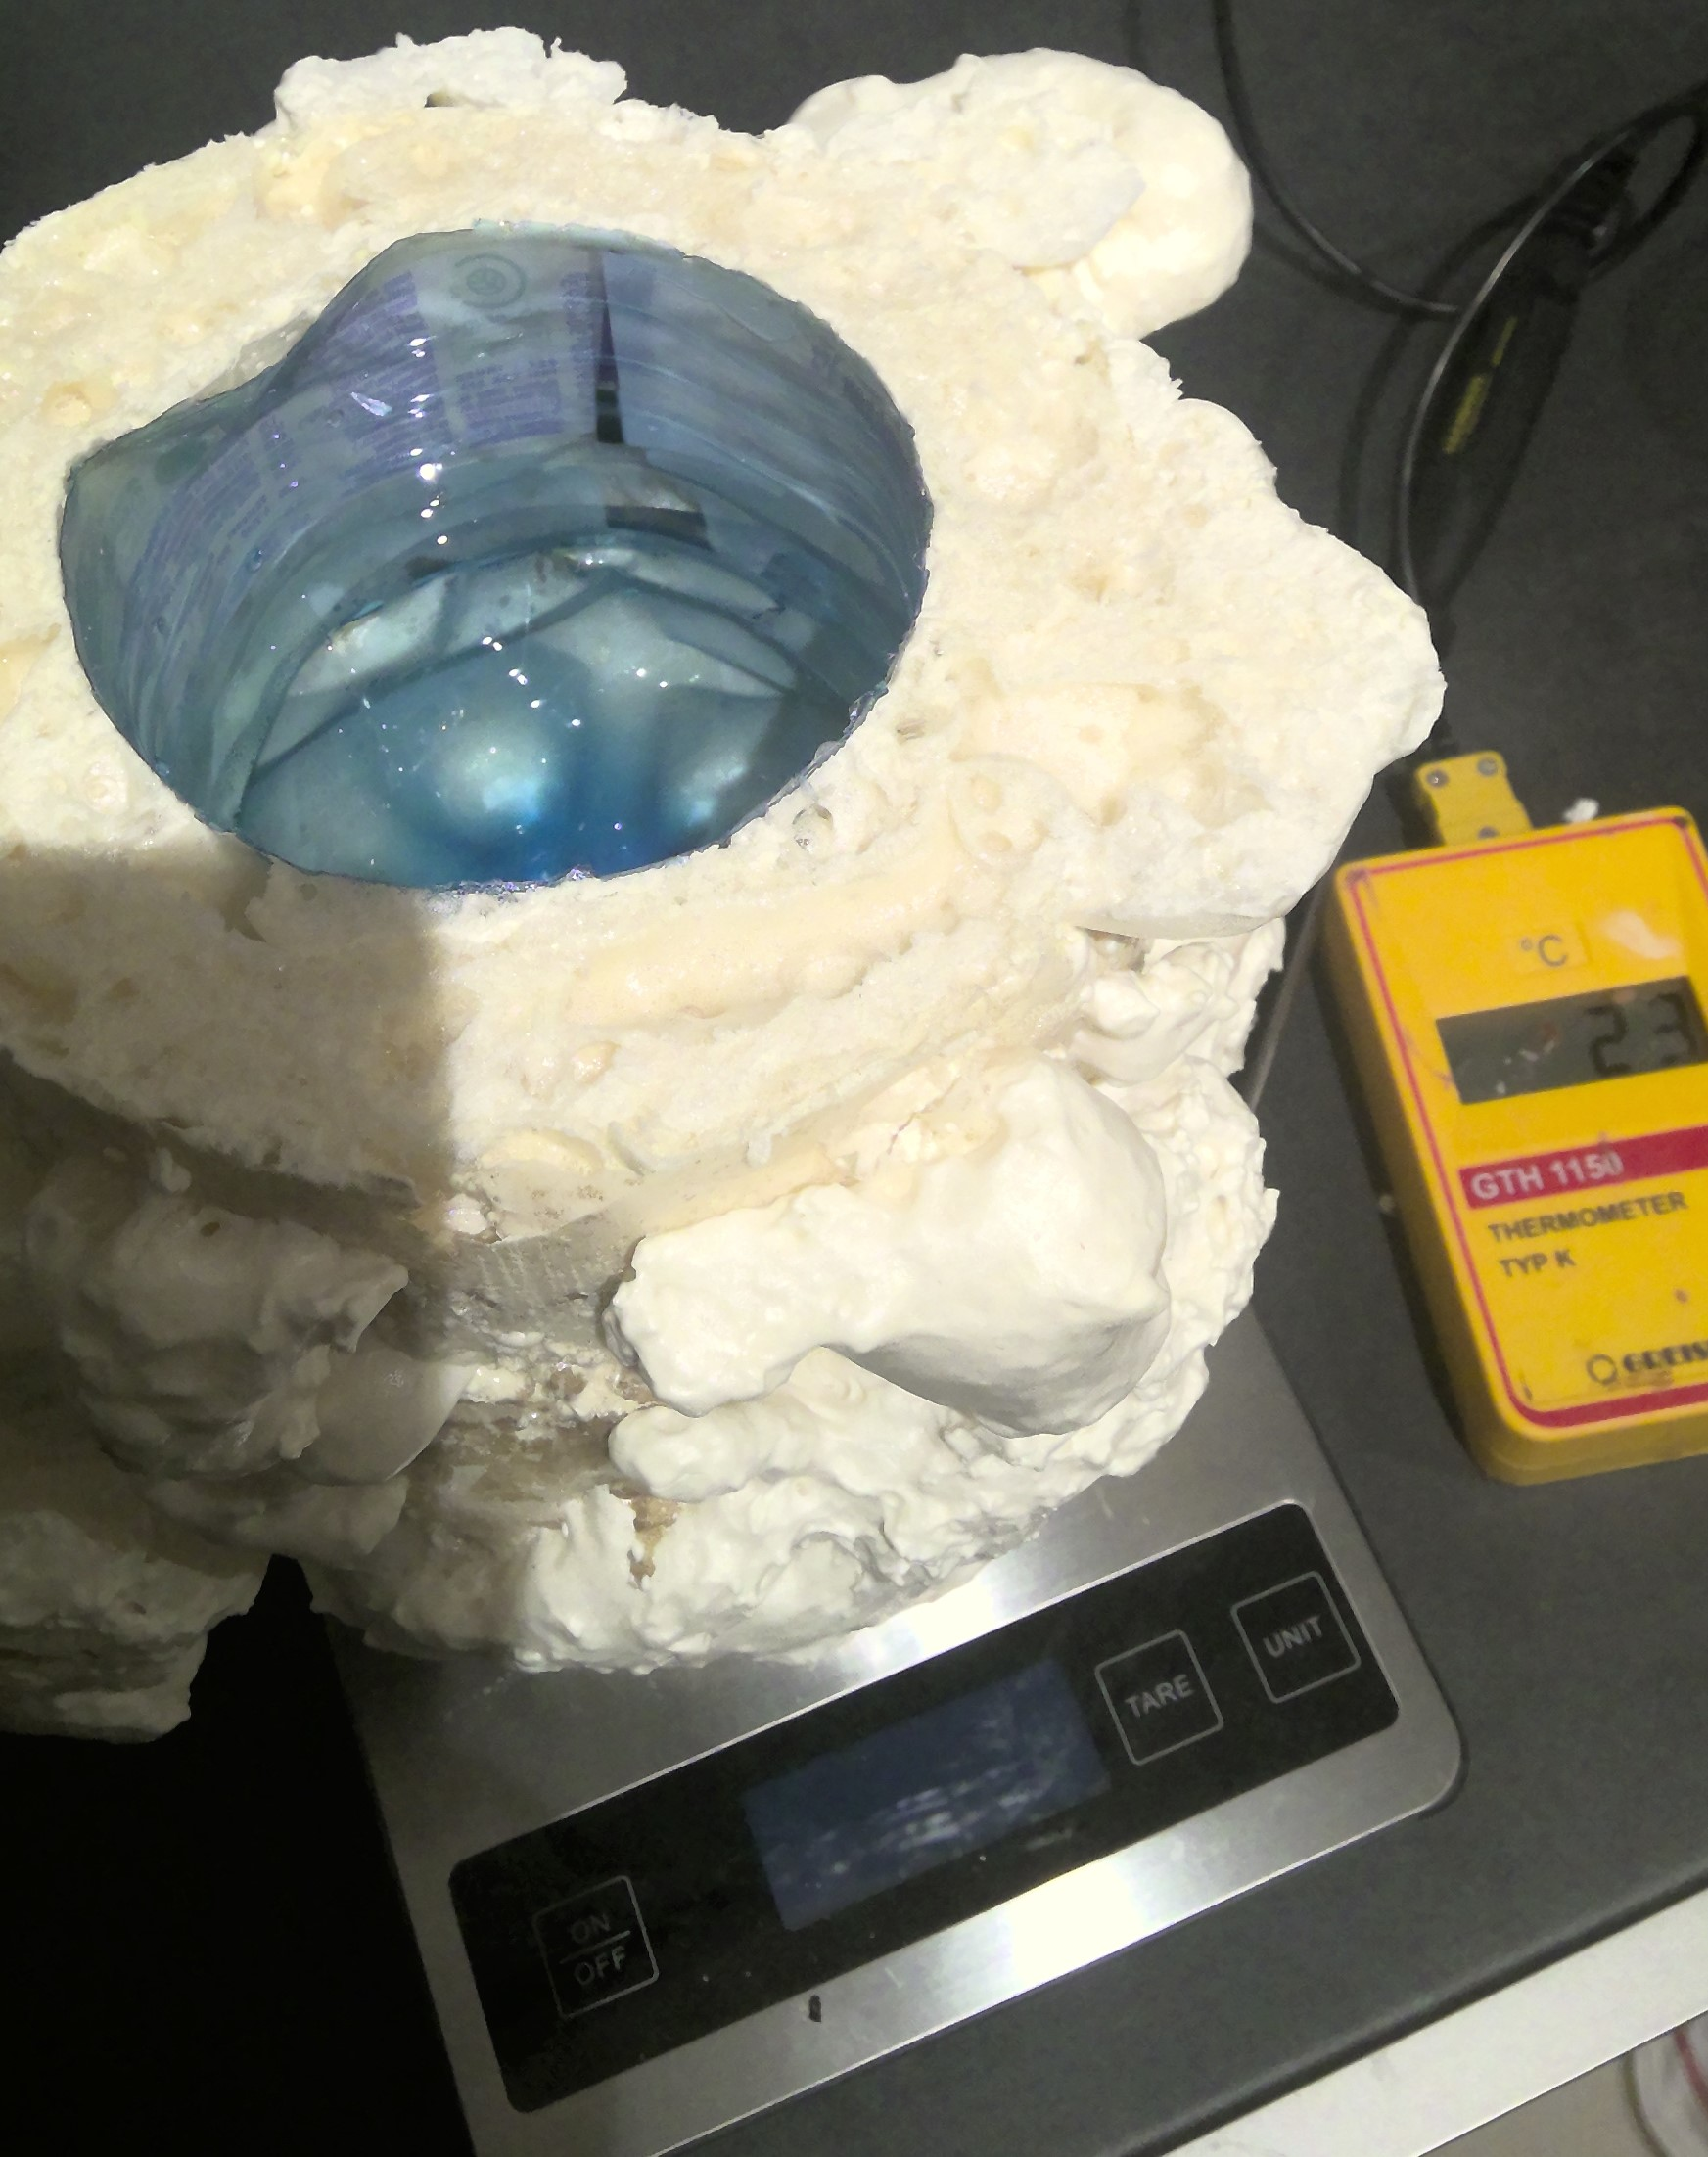
\includegraphics[width=\linewidth]{pics/Aufbau (1).jpg}
		\caption[Aufbau isoliertes Gefäß auf der Waage (Oben)]{Das isolierte Gefäß
			auf der Waage Perspektive von oben.}
		\label{fig:waageaufbau1}
	\end{minipage}
	\begin{minipage}[t]{.33\linewidth} % [b] => Ausrichtung an \caption
		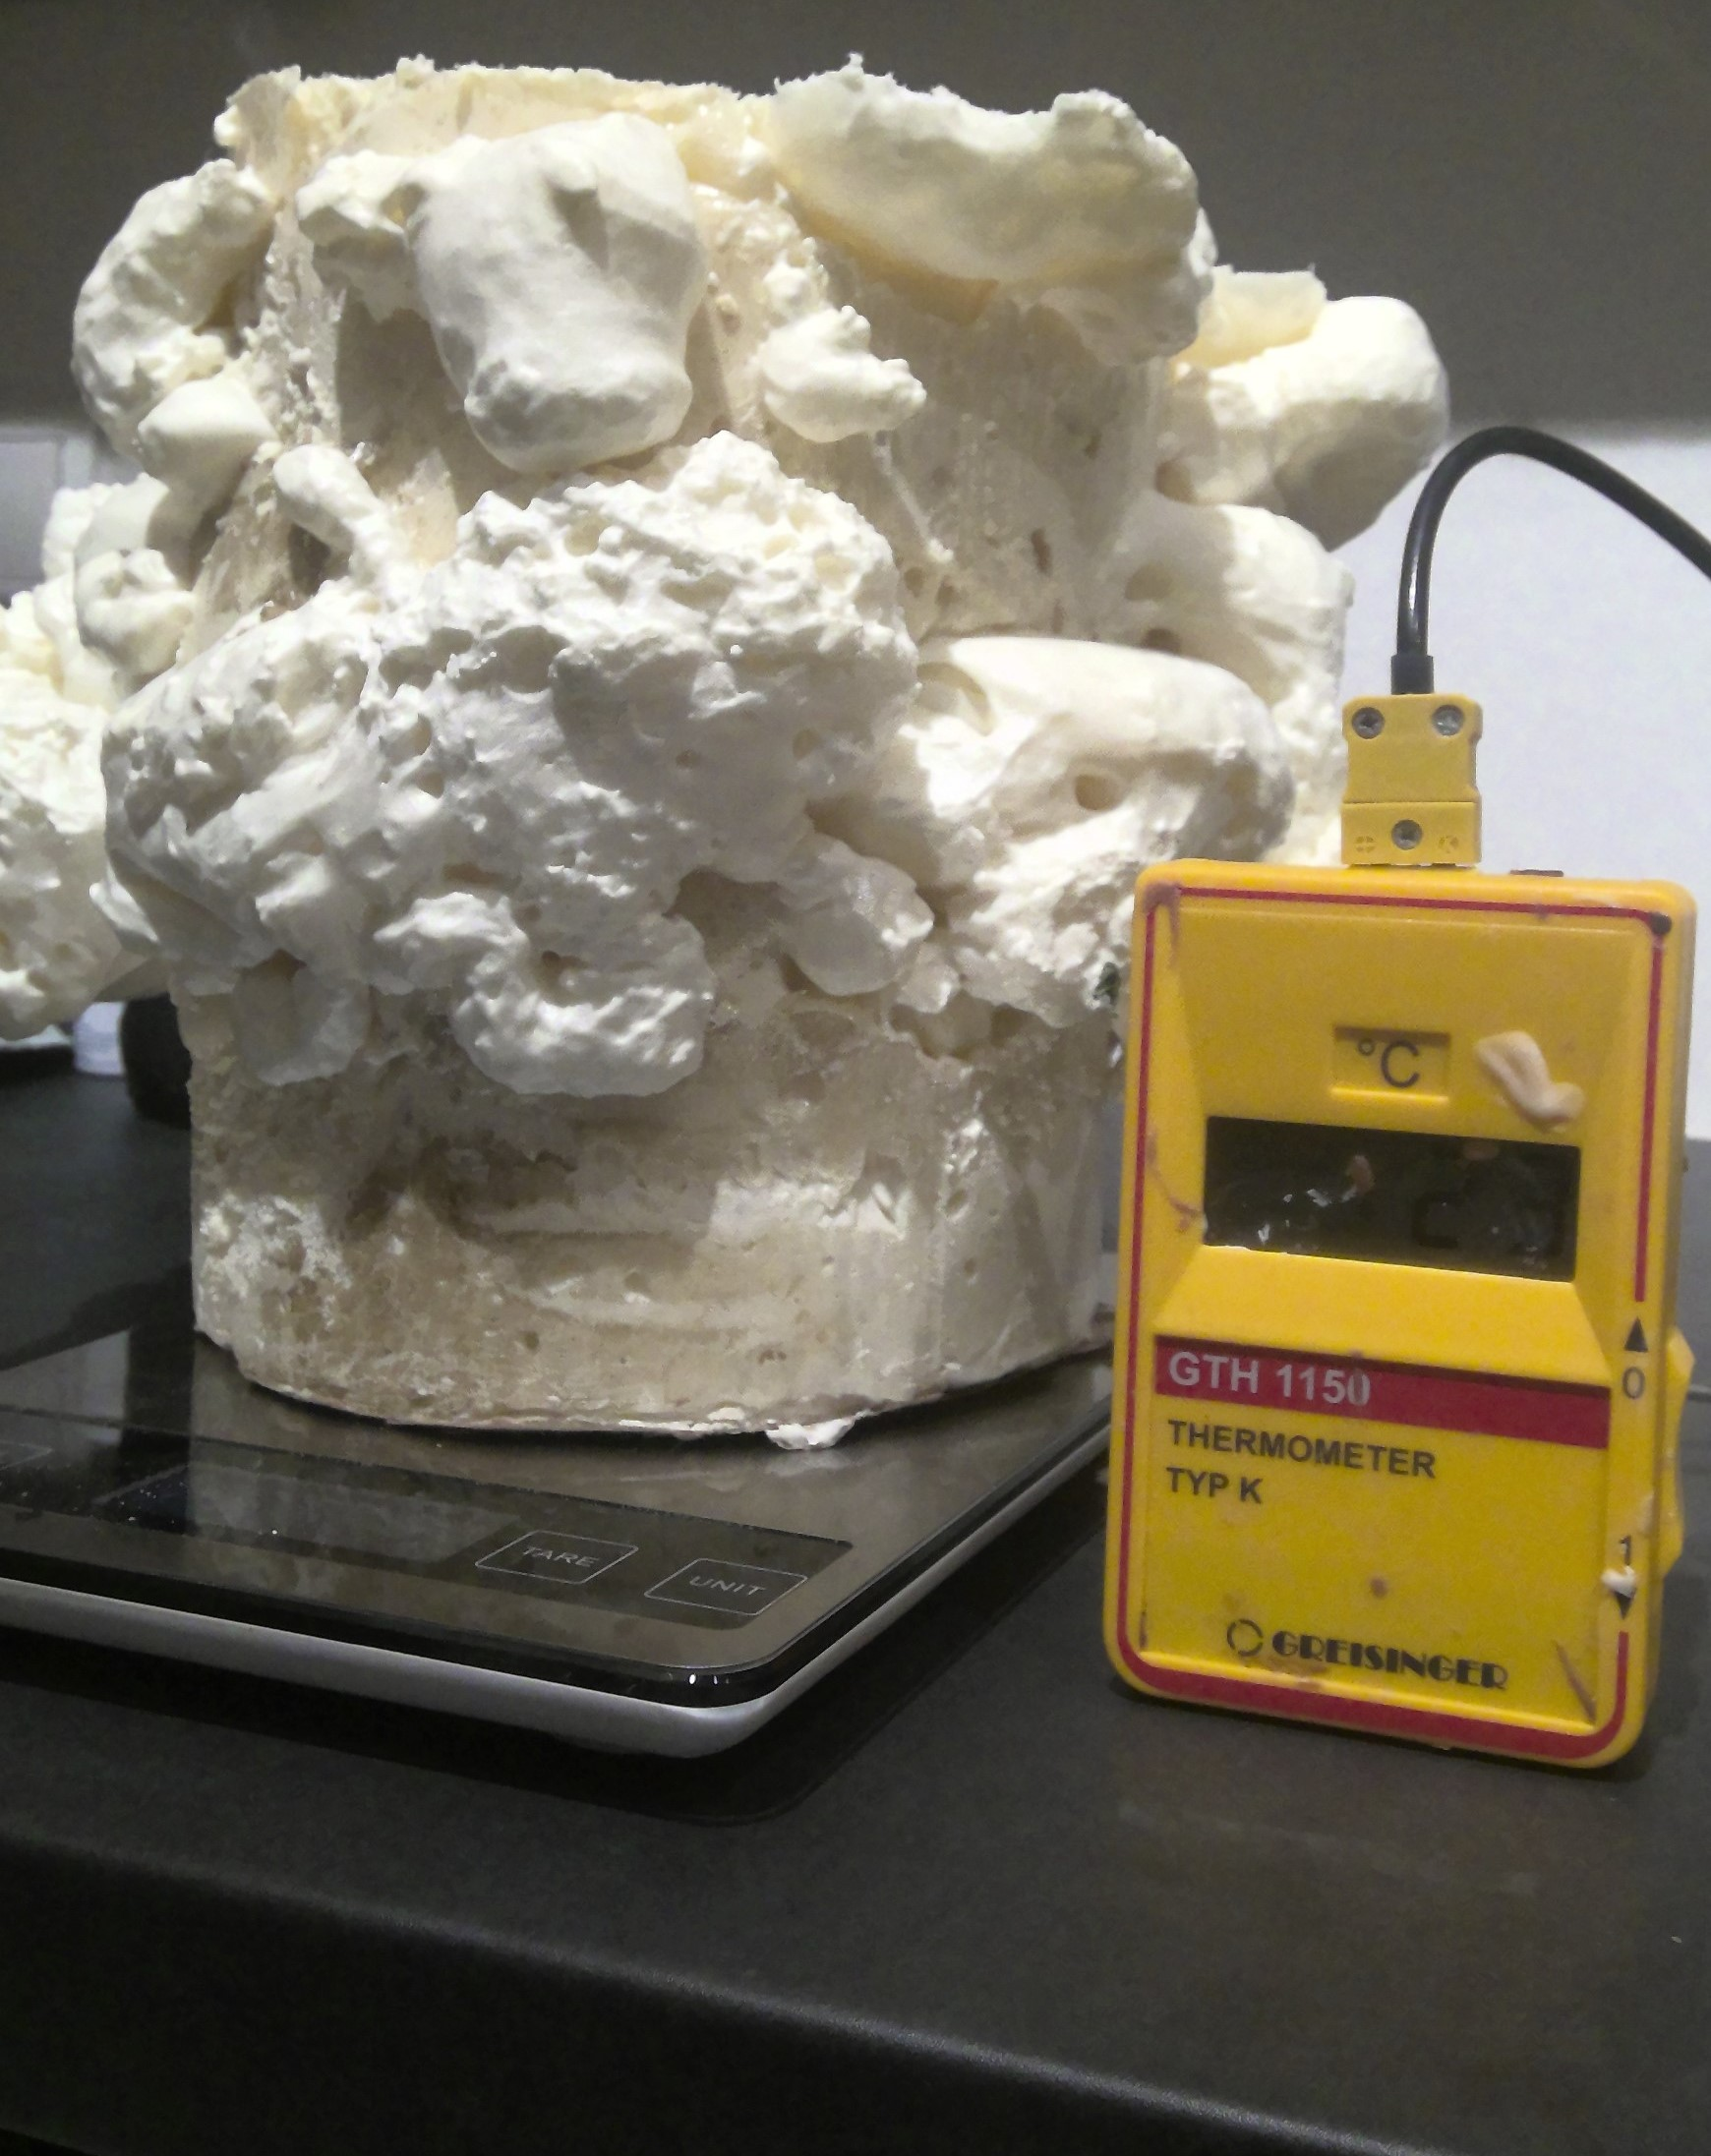
\includegraphics[width=\linewidth]{pics/Aufbau (2).jpg}
		\caption[Aufbau isoliertes Gefäß auf der Waage (Frontal)]{Das isolierte Gefäß
			auf der Waage Perspektive frontal.}
		\label{fig:waageaufbau2}
	\end{minipage}
	\begin{minipage}[t]{.30\linewidth} % [b] => Ausrichtung an \caption
		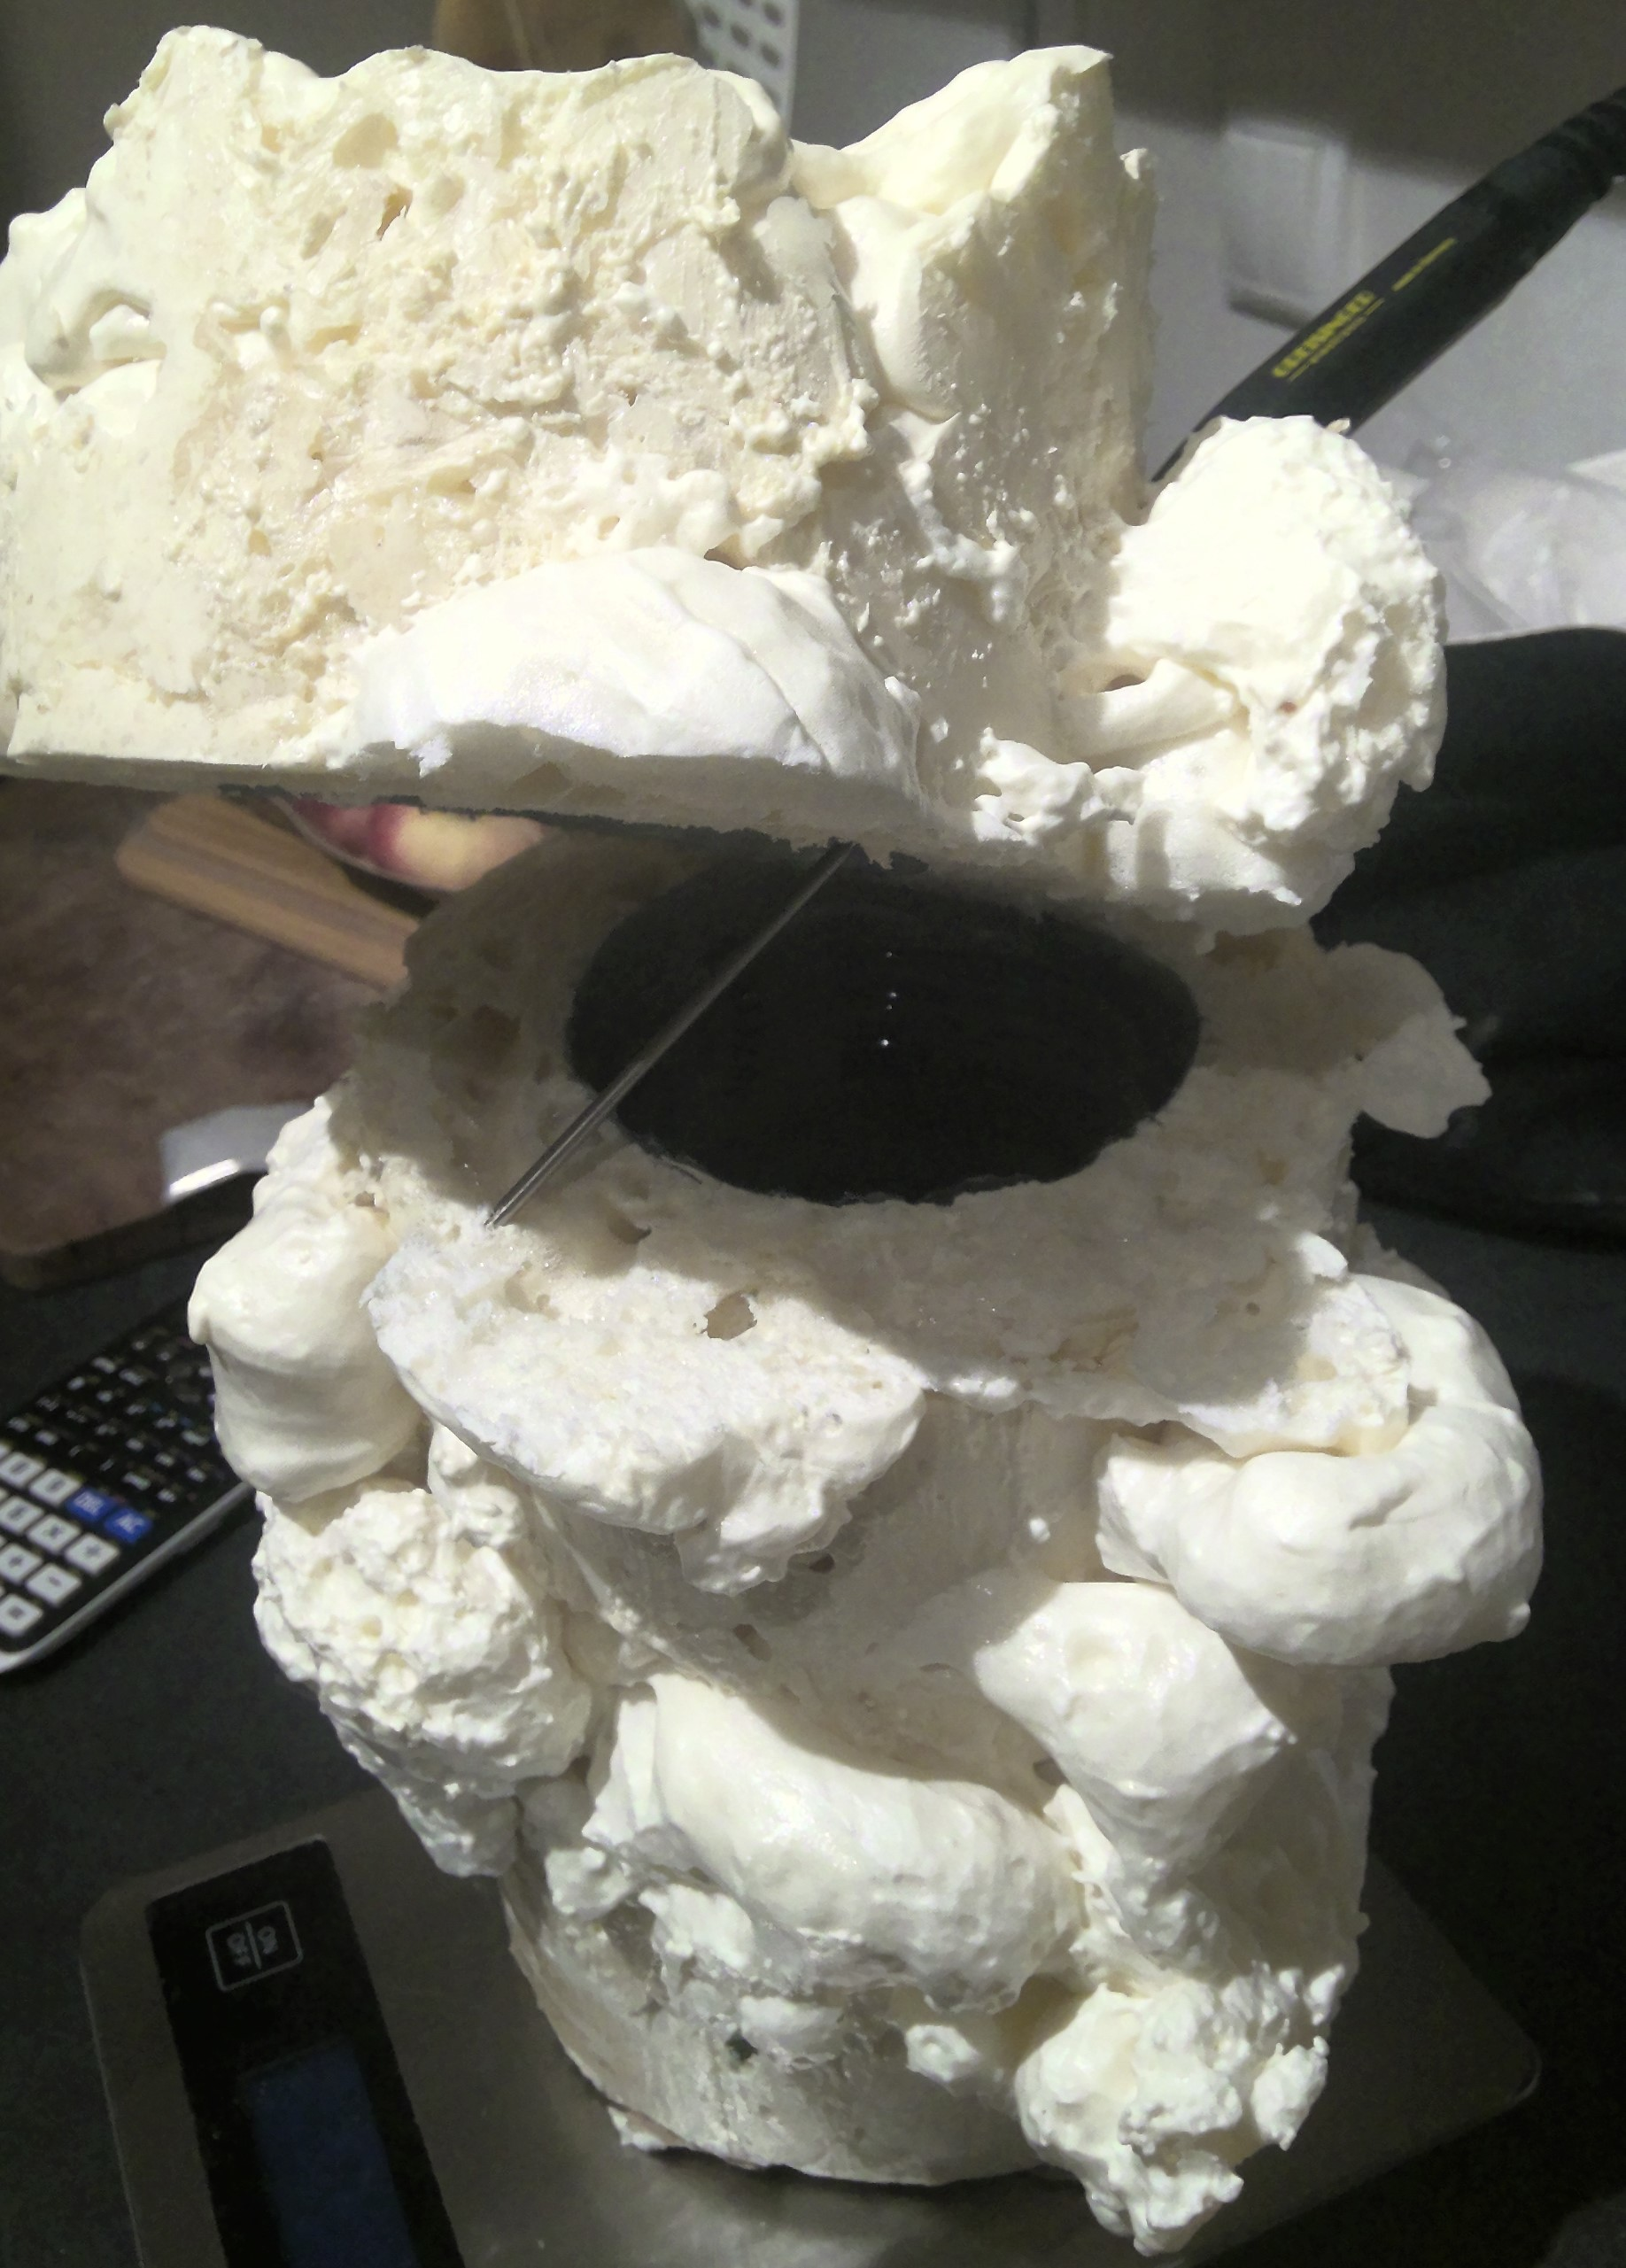
\includegraphics[width=\linewidth]{pics/Aufbau (3).jpg}
		\caption{Dieses Bild zeigt wie das Thermometer die Temperatur im Gefäß misst,
			wenn es geschlossen ist.}
		\label{fig:aufbauthermo}
	\end{minipage}
\end{figure}

\section{Geräteliste}
\label{sec:geraeteliste}
%\setlength\LTleft{-6.5em}
\begin{longtable}{c|c|S|p{19em}}
	\caption[Geräteliste]{Verwendete Geräte \label{tab:geraeteliste}}                                                                                                                               \\  % optionales Argument wird in Verzeichnissen verwendet, essentielles Argument direkt im Text
	\toprule
	Gerät          & Gerät-Nr. & { Unsicherheit }                    & Bemerkungen                                                                                                                  \\
	\midrule
	\endfirsthead
	\caption[]{(Fortsetzung)}                                                                                                                                                                       \\
	\toprule
	Gerät          & Gerät-Nr. & { Unsicherheit }                    & Bemerkungen                                                                                                                  \\
	\midrule
	\endhead
	\endfoot
	\endlastfoot

	Kartoffeln     & axx       & \SI{228(2)}{\g}                     & Ist das Material, von dem die Spezifische Wärmekapazität bestimmt wird                                                       \\ \hline
	Ethanol        & bxx       & { - }                               & Ist das Material, von dem die Spezifische Wärmekapazität bestimmt wird                                                       \\ \hline
	Waage          & cxx       & \SI{+-2}{\permille} +- 1 {Digit}    & Um die Masse der hinzufügten Flüssigkeiten und der diversen Stoffe zu messen                                                 \\ \hline
	Heizplatte     & dxx       & { - }                               & Zum Erhitzen des Wassers                                                                                                     \\ \hline
	Plastikflasche & gxx       & { - }                               & Wird verwendet um das Isolierte Gefäß zu bauen                                                                               \\ \hline
	PU-Schaum      & hxx       & { - }                               & Wird verwendet um das Isolierte Gefäß zu bauen                                                                               \\ \hline
	Thermometer    & jxx       & \SI{+-1}{\kelvin}\cite{thermometer} & Modell: GTH 1150 (Greisinger GmbH.) Um die Umgebungstemperatur und alle im Experiment zu messenden Temperaturen zu bestimmen \\ \hline

	\hline
\end{longtable}

\section{Versuchsdurchführung und Messergebnisse}
\label{sec:versuchsdurchfuehrung_messergebnisse}

\subsection{Bestimmung der Wärmekapazität des isolierten Gefäßes}
Für die Bestimmung der Wärmekapazität $C_K$ des Kalorimeters wird die
Umgebungstemperatur gemessen, welche der Temperatur des Wassers im isolierten
Gefäß und der Temperatur des Gefäßes selbst, entspricht. Nun wird das Wasser
erhitzt, in die isolierte Plastikflasche gegossen und dessen Temperatur gemessen.
Die Flüssigkeit wird durchmischt und das isolierte Gefäß geschlossen. Nun
wartet man ca. 10 Sekunden, bis der Temperaturaustausch stattgefunden hat. Nach
diesen 10 Sekunden wird die Flüssigkeit nochmals mit dem Thermometer umgerührt
und die Mischtemperatur gemessen.

\subsubsection{Ablauf}
\begin{enumerate}
	\item	Messen der Umgebungstemperatur, welche auch die Temperatur des Wassers im isolierten Gefäß und die Temperatur des Gefäßes ist
	\item	Erhitzen des zuzuführenden Wassers und Messen dessen Temperatur
	\item	Mischen der Flüssigkeiten und Schließen des isolierten Gefäßes
	\item	Warten bis der Temperaturaustausch stattgefunden hat; ungefähr 10s
	\item	Messen der Mischtemperatur, eventuell einmal mit der Probe umrühren
\end{enumerate}

\subsubsection{Werte}
Durch das Durchführen dieses Ablaufes sind folgende Messwerte entstanden, siehe
\autoref{tab:messwerte_gefass}:

\begin{table}[H]
	\centering
	\caption{In dieser Tabelle sind die notwendigen Messwerte um die
		Wärmekapazität des isolierten Gefäßes zu bestimmen. \\
		$T_U$ ist die Umgebungstemperatur \\
		$T_A$ ist die Temperatur des erhitzten Wassers \\
		$T_B$ ist die Temperatur des Gefäßes und des kalten, im Gefäß vorhandenen, Wassers \\
		$T_m$ ist die Mischtemperatur des gemischten Wassers \\
		$m_A$ ist die Masse des erhitzten Wassers \\
		$m_B$ ist die Masse des kalten, im Gefäß vorhandenen, Wassers \\
	}
	\label{tab:messwerte_gefass}
	\begin{tabular}{l|S|S}
		Symbol                  & {Werte} & {$\Delta$} \\ \hline
		$T_U$   / \si{\celsius} & 23      & +-1        \\
		$T_A$   / \si{\celsius} & 97      & +-1        \\
		$T_B$   / \si{\celsius} & 23      & +-1        \\
		$T_m$   / \si{\celsius} & 55      & +-1        \\
		$m_A$   / \si{\g}       & 386     & +-2        \\
		$m_B$   / \si{\g}       & 336     & +-2        \\ \hline
	\end{tabular}
\end{table}

\subsection{Bestimmung der spezifischen Wärmekapazität der diversen Stoffe}
Zur Bestimmung der spezifischen Wärmekapazität eines Stoffes, in diesem Fall ein
Ethanol und Kartoffeln, wird anfangs wieder die Umgebungstemperatur
bestimmt. Die Umgebungstemperatur entspricht der Temperatur des zu
untersuchenden Stoffes. Das zuzuführende Wasser wird erhitzt und in die
isolierte Plastikflasche gegossen. Nun wartet man 10 Sekunden, bis der
Temperaturaustausch stattgefunden hat und misst die Temperatur des erhitzten
Wassers und somit des isolierten Gefäßes. Jetzt wird der zu probende Stoff
hinzugefügt und man wartet erneut 10 Sekunden, bis der Flüssigkeitsaustausch
stattgefunden hat. Die Probe wird mit dem Thermometer umgerührt und die
Mischtemperatur wird gemessen.

\subsubsection{Ablauf}
\begin{enumerate}
	\item Umgebungstemperatur messen, welche auch die Temperatur des zu untersuchenden Stoffes ist
	\item Wasser erhitzen und in das isolierte Gefäß einfüllen
	\item 10s Temperaturaustausch von statten gehen lassen
	\item Temperatur des erhitzten Wassers und somit des isolierten Gefäßes messen
	\item Nun den zu probenden Stoff hinzufügen
	\item Warten bis der Temperaturaustausch stattgefunden hat; ungefähr 10s
	\item Messen der Mischtemperatur und einmal umrühren mit der Probe
\end{enumerate}

\subsubsection{Werte}
Durch das Durchführen dieses Ablaufes sind folgende Messwerte entstanden, siehe
\autoref{tab:messwerte_stoffe}:

\begin{table}[H]
	\centering
	\caption{In dieser Tabelle sind die notwendigen Messwerte um die
		spezifische Wärmekapazität von Ethanol ($E$) und Kartoffeln ($K$) zu bestimmen. \\
		$T_U$ ist die Umgebungstemperatur \\
		$T_A$ ist die Temperatur des zu untersuchenden Materials gleich der Umgebungstemperatur \\
		$T_B$ ist die Temperatur des Gefäßes und des erhitzten, im Gefäß vorhandenen, Wassers \\
		$T_m$ ist die Mischtemperatur des gemischten Wassers \\
		$m_A$ ist die Masse des zu untersuchenden Stoffes \\
		$m_B$ ist die Masse des erhitzten, im Gefäß vorhandenen, Wassers \\
	}
	\label{tab:messwerte_stoffe}
	\begin{tabular}{l|S|S}
		Kartoffeln             & {Werte} & {$\Delta$} \\ \hline
		$T_U$ / \si{\celsius}  & 23      & 1          \\
		$T_A$ / \si{\celsius}  & 11      & 1          \\
		$T_B$ / \si{\celsius}  & 81      & 1          \\
		$T_m$ / \si{\celsius}  & 66      & 1          \\
		$m_A$ / \si{\g}        & 182     & 2          \\
		$m_B$ / \si{\g}        & 318     & 2          \\ \hline \hline
		Ethanol                & {Werte} & {$\Delta$} \\ \hline
		$T_U$  / \si{\celsius} & 23      & 1          \\
		$T_A$  / \si{\celsius} & 22      & 1          \\
		$T_B$  / \si{\celsius} & 92      & 1          \\
		$T_m$  / \si{\celsius} & 69      & 1          \\
		$m_A$  / \si{\g}       & 289     & 2          \\
		$m_B$  / \si{\g}       & 145     & 2          \\ \hline
	\end{tabular}
\end{table}

Die Kartoffeln wurden klein gehackt.

\section{Auswertung}
\label{sec:auswertung}

Verwendet man nun den Wert für die spezifische Wärmekapazität für
Wasser $c_W$ = \SI{4187}{\joule\per\kg\kelvin} \cite{Ahrberg2011}
und die gemessenen Werte, aus \autoref{tab:messwerte_gefass} in \autoref{eq:warmegefaes}, so
erhält man folgenden Wert für die Wärmekapazität des
Gefäßes:

\begin{equation}
	C_K = \SI{230(130)}{\joule\per\kelvin}
\end{equation}

Verwendet man nun den Wert für die spezifische Wärmekapazität für
Wasser $c_W$ = \SI{4187}{\joule\per\kg\kelvin} \cite{Ahrberg2011}
und die gemessenen Werte, aus \autoref{tab:messwerte_stoffe} in \autoref{eq:warmestoff},
erhält man folgende Werte für die Wärmekapazität der
Stoffe:

\begin{equation}
	c_{Kartoffeln}   = \SI{}{\joule\per\kg\kelvin}
	c_{Ethanol} = \SI{}{\joule\per\kg\kelvin}
\end{equation}

Wobei $c_{Kartoffeln}$ und $c_{Ethanol}$ die gemessen
Wärmekapazitäten von Kartoffeln und Ethanol sind.


\section{Diskussion und Zusammenfassung}
\label{sec:diskussion_zusammenfassung}
% Aufzählung was scheiße glaufen is

Nun werden die verwendeten Methoden diskutiert und die Ergebnisse
zusammengefasst.

\subsection{Diskussion}

Bei der Bestimmung der Wärmekapazität des Gefäßes
ist aufgrund der ungenauen Temperaturbestimmung
kein Akkuraterwert bestimmt worden. Dennoch lässt
sich sagen, dass der Wert \SI{230(130)}{\joule\per\kelvin} größenordnungsmäßig
dem Wert von einem gut isolierenden Gefäß \SIrange{100}{200}{\joule\per\kelvin} \cite{wärmehinweise} entspricht.

Um den Fehler bei dem Umfüllen zu minimieren, wurde
die Distanz zwischen der Wasseroberfläche im isolierten
Gefäß und dem Rand des Wasserkochers minimiert, weiters
ist versucht worden den Fluss laminar zu machen, damit
keine Luftblasen im Wasser sind.

Wie auch bei den Hinweisen \cite{wärmehinweise} erwähnt, waren hier
große Fehlermargen zu erwarten.

Bei der Bestimmung der spezifischen Wärmekapazität der Stoffe
ist die Fehlerquelle des Umfüllens nicht vorhanden, da
sich das Wasser schon im isolierten Gefäß befindet und
die zu untersuchenden Materialien hinzugefügt werden.

Beim Bestimmen der spezifischen Wärmekapazität von Ethanol
ist zu beachten, dass die Siedetemperatur von Ethanol \cite{isopropanolsiede}
niedriger als die von Wasser ist und somit die Temperatur vom Wasser
bestenfalls unter der Siedetemperatur von Ethanol liegt. Dies
wurde jedoch berücksichtigt.

Die Werte für die spezifischen Wärmekapazitäten beinhalten
die Literaturwerte in ihren Unsicherheitsintervallen und haben einen nicht
so hohen
relativen Fehler \SI{10}{\percent}, siehe \autoref{tab:ergebnisse}.
Ein Erklärung für die Diskrepanz zwischen dem gemessen Wert der
spezifischen Wärmekapazität von Kartoffeln und dem
theortischen Wert, könnte sein Aufgrund
der Zerteilung der Kartoffeln sein. Da der Wärmeaustausch
dann schneller von statten gehen kann und somit das System
schneller im Equilibrium ist. Werden jedoch
ganze Kartoffeln genommen kann man Werte man niedrigere
Werte für die spezifische Wärmekapazität finden, wenn
der gesamte Energieaustausch von stattengegangen ist.


\begin{table}[H]
	\centering
	\caption{Hier werden die erhaltenen Werte den Literaturwerten gegenübergestellt.\\
		$c_{Kartoffeln}$ Die spezifische Wärmekapazität von Kartoffeln\\
		$c_{Ethanol}$ Die spezifische Wärmekapazität von Ethanol \\
		$C_{K}$ Die Wärmekapazität von dem isolierten Gefäß \\
		Alle Werte wurden unter folgenden Bedingungen aufgenommen: \\
		Umgebungstemperatur @ \SI{23(1)}{\celsius} \\
		Luftdruck @ \SI{1013.25}{\hecto\pascal} \\
	}
	\label{tab:ergebnisse}
	\begin{tabular}{c|S|S|S}
		Symbol:                                           & {Bestimmter Wert} & {Literaturwert}                          & {Literaturwert}                \\ \hline
		$c_{Kartoffeln} / \si{\joule\per\kg\per\kelvin} $ & 4900(500)         & 3390 \cite{kartoffel2}                   & 3430 \cite{kartoffelkapazität} \\
		$c_{Ethanol}$ / \si{\joule\per\kg\per\kelvin}     & 2340(270)         & 2428 \cite{ethanolkapazitat}             &                                \\
		$C_{K}$ / \si{\joule\per\kelvin}                  & 230(130)          & \numrange{100}{200} \cite{wärmehinweise} &                                \\
	\end{tabular}
\end{table}

\subsection{Zusammenfassung}

Da bei allen erhaltenen Werten die Literaturwerte im Fehlerintervall enthalten sind, lässt
sich sagen, dass die Methoden zureichend sind, um diese Werte größenordnungsmäßig
zu bestimmen. Wenn die Auswertung richtig gemacht wurde, sind auch die relativen
Unsicherheiten der spezifischen Wärmekapazitäten nicht exorbitant. Im Ganzen
lässt sich sagen, dass dieses Experiment die Literaturwerte weiter unterstützt.

Ein Verbesserungsvorschlag wäre, wenn die Werte noch genauer bestimmt werden
müssen, genauere Messgeräte zu verwenden. Weiters wäre es
gut ein noch größeres isoliertes Gefäß zu bauen, damit man
mit größeren Massen leichter umgehen kann.
% Literaturtabelle
\newpage
\printbibliography

\listoffigures

\listoftables


\end{document}
